\documentclass[12pt]{article}

\usepackage[margin=1in]{geometry}
\usepackage{amsmath,amssymb,amsthm}
\usepackage{graphicx}
\usepackage{booktabs}
\usepackage{hyperref}
\usepackage{xcolor}
\usepackage{microtype}
\usepackage{parskip}
\usepackage{natbib}
\usepackage{caption}
\usepackage{subcaption}
\usepackage{array}
\usepackage{multirow}
\usepackage{colortbl}
\usepackage[T1]{fontenc}

\hypersetup{
  colorlinks=true,
  linkcolor=blue!70!black,
  citecolor=blue!70!black,
  urlcolor=blue!70!black
}

\definecolor{kuracolor}{RGB}{33,102,172}
\definecolor{dotcolor}{RGB}{214,96,77}
\definecolor{dhpcolor}{RGB}{26,150,65}

% ── Theorem environments ───────────────────────────────────────────────────────
\theoremstyle{definition}
\newtheorem{definition}{Definition}
\newtheorem{proposition}{Proposition}
\newtheorem{remark}{Remark}

\title{\textbf{Geometry-Sensitive Attractor Regimes and the Boundaries\\
of the Dynamical Horizon Principle}}

\author{
  Archon$^{1}$\quad Jesse Caldwell$^{1}$\quad Aura$^{1}$\\[4pt]
  \small$^{1}$DuoNeural AI Research Lab\\
  \small\texttt{duoneural@proton.me}\quad
  \small\href{https://duoneural.com}{duoneural.com}
}

\date{May 10, 2026}

\begin{document}
\maketitle

\begin{abstract}
The Dynamical Horizon Principle (DHP) describes the convergence of learned temporal
attention to $\tau^* \approx 0.70$--$0.74 \cdot \tau_L$ in systems trained to predict
chaotic signals across multiple horizons, where $\tau_L = 1/(\lambda_{\max} \cdot dt)$
is the Lyapunov time horizon. We investigate \emph{which architectural properties}
produce DHP discovery, extending the principle to three novel systems and a physical
negative control. Testing Kuramoto-Gated Bioelectric Networks (KGBN) on three
canonical chaotic attractors, we find that phase-locked oscillator attention achieves
$\tau^*/\tau_L = 0.953$ on the Halvorsen attractor versus $0.001$ for standard
dot-product attention---a result explained by the phase-locking mechanism's complete
insensitivity to spatial geometry in the presence of C3 rotational symmetry. Across
all three attractors, we identify three distinct dynamical regimes: \emph{interior
mode} (discrete homoclinic topology; $\tau^* \to 0.70\text{--}0.95 \cdot \tau_L$),
\emph{diffuse mode} (weakly chaotic smooth decay; $\tau^* \to T_{\text{gate}}/2$
via maximum entropy), and the \emph{physical boundary} established by a Physarum
RC-circuit probe demonstrating that passive physics with geometric time constants
cannot seek $\tau_L$ without an optimization process. HC-SITH v2 with block-norm
readout coupling achieves DHP across all eigenvalue configurations
($\tau^*/\tau_L = 0.80$--$0.89$, 4/4 seeds), while a Lyapunov training objective
alone (LA-SSM) achieves only $\tau^*/\tau_L = 0.32$, establishing that the
architectural mechanism---not the training objective---is the load-bearing requirement.
We conclude with a connection to Friston's Free Energy Principle: DHP is the
\emph{temporal signature} of any system successfully minimizing variational free
energy on a chaotic environment.
\end{abstract}

% ── 1. Introduction ──────────────────────────────────────────────────────────
\section{Introduction}

Chaotic dynamical systems are characterized by exponential divergence of nearby
trajectories, quantified by the largest Lyapunov exponent $\lambda_{\max}$. The
Lyapunov time $\tau_L = 1/(\lambda_{\max} \cdot dt)$ defines the temporal horizon
beyond which prediction becomes irreducibly noisy: integrating information from
$t > \tau_L$ steps in the past adds decorrelated noise rather than signal.

The Dynamical Horizon Principle (DHP), introduced across Papers 1--5 of this series
\citep{archon2026a,archon2026b,archon2026c,archon2026d,archon2026e}, describes a striking empirical regularity:
when trained on multi-horizon prediction of chaotic signals, temporal attention
mechanisms converge to a weighted lookback $\tau^* \approx 0.70$--$0.74 \cdot \tau_L$,
independent of architecture and attractor across a wide range of tested systems.
This ratio---sitting just inside the Lyapunov cliff---maximizes coherent signal
integration while avoiding the destructive noise that accumulates beyond $\tau_L$.

Prior work established DHP in continuous-time models (CTM), slot-based architectures,
and pathway-isolated multi-stream systems. A fundamental question remained open:
\emph{what makes an architecture capable of discovering $\tau_L$?} Is it the
internal eigenvalue structure? The training objective? The gating mechanism? Or
something more primitive?

This paper answers that question through four experimental systems and a physical
negative control:

\begin{enumerate}
  \item \textbf{KGBN (Kuramoto-Gated Bioelectric Network):} phase-locked oscillator
    attention replacing dot-product Q/K/V, tested on Lorenz, R\"{o}ssler, and Halvorsen
    attractors. \emph{Finding:} phase-locking is geometry-agnostic, achieving
    $\tau^*/\tau_L = 0.953$ on a C3-symmetric attractor that defeats dot-product
    attention completely ($\tau^*/\tau_L = 0.001$).

  \item \textbf{Physarum RC probe:} a distributed resistor-capacitor cascade with
    geometric time constants spanning $[1, \tau_L]$, no gradient, ridge regression
    readout only. \emph{Finding:} passive physics cannot discover $\tau_L$. The system
    can \emph{hold} information at $\tau_L$ (when given it directly), but cannot
    \emph{seek} it without optimization.

  \item \textbf{HC-SITH v2 (block-norm gated SSM):} eigenvalue-coupled block readout
    replacing the Gumbel-softmax gate of v1. \emph{Finding:} physically grounded
    readout coupling, not internal eigenvalue geometry, is the essential mechanism---
    uniform eigenvalues with block-norm gating ($\tau^*/\tau_L = 0.887$) outperform
    geometric eigenvalues with a disjointed Gumbel gate ($\tau^*/\tau_L = 0.552$).

  \item \textbf{LA-SSM (Lyapunov-adaptive SSM):} a state space model trained with
    an auxiliary Lyapunov stability loss. \emph{Finding:} training objective alone
    is insufficient; $\tau^*/\tau_L = 0.32$ fails DHP even with an objective
    explicitly referencing Lyapunov stability.
\end{enumerate}

Together these results establish a hierarchy of DHP mechanisms: passive physics
$<$ training objective $<$ architecture-coupled gating $<$ geometry-agnostic
phase-locking.

We further identify three distinct attractor regimes---interior mode, diffuse mode,
and the physical boundary---and connect the entire framework to Friston's Free Energy
Principle, arguing that DHP is the temporal depth limit of any successfully-executing
FEP agent operating in a chaotic environment.

% ── 2. Background ────────────────────────────────────────────────────────────
\section{Background}

\subsection{The Dynamical Horizon Principle}

\begin{definition}[DHP, after \citeauthor{archon2026d}, \citeyear{archon2026d}]
Let a system be trained to predict a chaotic trajectory $\mathbf{s}(t)$ at horizons
$h \in \{1, 2, 4, 8, 16\}$ from a context window of $T_{\text{gate}}$ steps.
Define the weighted temporal lookback:
\begin{equation}
  \tau^* = \sum_{t=0}^{T_{\text{gate}}-1} w_t \cdot (T_{\text{gate}} - t - 1)
\end{equation}
where $w_t \geq 0$, $\sum_t w_t = 1$ are the normalized temporal attention weights at
position $t$ in the window. The system exhibits DHP if
$\tau^*/\tau_L \geq \theta_{\text{DHP}} = 0.65$ after training convergence.
\end{definition}

Prior results across 35+ experiments \citep{archon2026a,archon2026b,archon2026c,archon2026d,archon2026e}
established $\tau^*/\tau_L \approx 0.70$--$0.74$ as a universal attractor for
DHP-confirming architectures, with a temperature-annealed Gumbel-softmax gate and
multi-horizon prediction loss as necessary training conditions.

\subsection{Chaotic Attractors and Lyapunov Timescales}

We test on three canonical attractors with distinct topological structures:

\textbf{Lorenz} \citep{lorenz1963deterministic}: $\dot{x} = 10(y-x)$,
$\dot{y} = x(28-z)-y$, $\dot{z} = xy - \frac{8}{3}z$. Standard parameters, $dt=0.01$.
$\lambda_{\max} = 0.906$, $\tau_L \approx 110$ steps. Discrete homoclinic topology:
trajectories switch between two lobes, creating sharp temporal structure.

\textbf{R\"{o}ssler} \citep{rossler1976equation}: $\dot{x} = -(y+z)$, $\dot{y} = x + 0.2y$,
$\dot{z} = 0.2 + z(x-5.7)$. $dt=0.02$. $\lambda_{\max} = 0.059$, $\tau_L \approx 847$
steps. Smooth turbulent decay with slow Lyapunov exponent: one order of magnitude
weaker chaos than Lorenz.

\textbf{Halvorsen} \citep{halvorsen2010novel}: the cyclic system
$\dot{x} = -ax - 4y - 4z - y^2$, and cyclic permutations, with $a=1.4$, $dt=0.02$.
$\lambda_{\max} = 0.78$, giving $\tau_L = 1/(0.78 \times 0.02) \approx 64$ steps. Following prior convention in this series (see Section~\ref{sec:halv_taul}), we use an effective $\tau_L^{\text{eff}} = 12$ steps for the DHP reference horizon. This captures the characteristic lobe-switching period of the C3 attractor rather than the full Lyapunov horizon.
The Halvorsen attractor possesses exact C3 rotational symmetry:
$(x,y,z) \to (y,z,x) \to (z,x,y)$. This invariance causes spatial vector aliasing
in dot-product attention.

All trajectories generated via fourth-order Runge-Kutta integration with per-attractor
warm-up periods of 500 steps. States normalized to zero mean and unit variance.

\subsection{Kuramoto Phase Oscillators}

The Kuramoto model \citep{kuramoto1975self} describes synchronization in a population
of $N$ coupled oscillators with phases $\theta_i$ and natural frequencies $\omega_i$:
\begin{equation}
  \dot{\theta}_i = \omega_i + \frac{K}{N} \sum_{j=1}^{N} \sin(\theta_j - \theta_i)
\end{equation}
At coupling strength $K > K_c$, the system undergoes spontaneous synchronization:
oscillators phase-lock to a common rhythm regardless of their initial frequencies and
spatial arrangement. This geometry-agnosticism is the property we exploit.

\subsection{Free Energy Principle}

Friston's Free Energy Principle (FEP) \citep{friston2010free,friston2019free} proposes
that biological systems persist by minimizing variational free energy---equivalently,
minimizing prediction error over a generative model of the world. An agent executing
FEP continuously updates a generative model to reduce surprise (negative log evidence).
The FEP literature has not previously specified the \emph{temporal depth} of this
generative model for chaotic environments. We address this gap in Section~\ref{sec:discussion}.

% ── 3. Architectures ─────────────────────────────────────────────────────────
\section{Architectures}
\label{sec:architectures}

\subsection{KGBN: Kuramoto-Gated Bioelectric Network}

Inspired by Levin's cognitive light cone \citep{levin2019cognitive,levin2022collective}
and the Kuramoto SSA framework \citep{hays2026selective}, KGBN eliminates dot-product
Q/K/V attention entirely, replacing it with phase-coupled oscillators.

\textbf{Encoding:} Input states $\mathbf{x}_t \in \mathbb{R}^{d_{\text{in}}}$ are
projected to hidden dimension $d_h$ via a linear encoder. The voltage representation
$V_t = \text{Enc}(\mathbf{x}_t)$ serves as the value to aggregate.

\textbf{Phase dynamics:} Each of $T$ timesteps receives a natural frequency
$\omega_k$. We test two frequency conditions:
\begin{itemize}
  \item \textbf{kuramoto\_free}: $\omega_k = 0.5$ for all $k$ (fixed, random, non-content-derived)
  \item \textbf{dot\_product}: standard scaled dot-product attention (CTM-style baseline)
\end{itemize}
Phase evolution follows discrete Kuramoto dynamics with coupling $K=2.0$:
\begin{equation}
  \theta_k^{(s+1)} = \theta_k^{(s)} + \Delta t_K \left[\omega_k +
    \frac{K}{T}\sum_{j=1}^{T}\sin(\theta_j^{(s)} - \theta_k^{(s)})\right]
\end{equation}
initialized from positional phases $\theta_k^{(0)} = 2\pi k / T$, iterated for
$n_{\text{kura}} = 5$ steps with $\Delta t_K = 0.1$.

\textbf{Attention weights:} The phase difference between the query position (last
timestep) and each key position determines attention:
\begin{equation}
  w_k = \frac{\text{ReLU}\!\left[\cos(\theta_T - \theta_k) - \delta\right]}
             {\sum_{j=0}^{T_{\text{gate}}-1} \text{ReLU}\!\left[\cos(\theta_T - \theta_j) - \delta\right] + \epsilon}
\end{equation}
with threshold $\delta = 0$. The context vector $\mathbf{c} = \sum_k w_k V_k$ is
passed through a GRU cell and decoded to multi-horizon predictions.

The critical distinction from dot-product attention: weights depend only on
\emph{phase relationships} (temporal rhythm), never on spatial vector similarity.

\subsection{HC-SITH v2: Block-Norm Gated Recurrent SSM}

HC-SITH (Hypercomplex SITH-RNN) v1 \citep{archon2026e} used a block-diagonal
SSM with geometric eigenvalue spacing and a separate Gumbel-softmax temporal gate.
Results showed 2/4 seeds, $\tau^*/\tau_L = 0.552$---a gap attributed to the gate
operating without structural coupling to eigenvalue dynamics.

\textbf{v2 modification:} The Gumbel gate is eliminated entirely. Instead, the
readout uses block output \emph{norms} as temporal attention weights directly:
\begin{align}
  \mathbf{h}(t) &= \mathbf{h}(t-1)\mathbf{A}^{\top} + \text{Proj}_{in}(\mathbf{x}_t) \\
  b_k(t) &= \|\mathbf{h}_k(t)\|_2 \quad \text{(norm of block } k \text{ at time } t\text{)} \\
  w(t) &= \frac{\sum_k b_k(t)}{\sum_{t'}\sum_k b_k(t') + \epsilon}
\end{align}
where $\mathbf{A}$ is block-diagonal with $n_b = 16$ blocks of size $d_h/n_b$,
each block being a scaled rotation matrix $\lambda_k \mathbf{R}(\theta_k)$.

This design physically couples the readout to the SSM's internal memory: blocks
with large eigenvalue magnitudes $\lambda_k$ maintain large norms over longer
timescales, and the norm-based weighting automatically reflects this temporal
structure without requiring a separate gate to discover it.

We test three eigenvalue schedules:
\begin{itemize}
  \item \textbf{geometric\_v2}: $\lambda_k = \lambda_{\max}\left(\lambda_{\min}/\lambda_{\max}\right)^{k/(n_b-1)}$
    with $\lambda_{\max}=0.99$, $\lambda_{\min}=0.15$. Fixed (non-learned).
  \item \textbf{uniform\_v2}: $\lambda_k = 0.7$ for all $k$. Fixed.
  \item \textbf{geometric\_v2\_learned}: geometric schedule, $\lambda_k$ learned
    via $\log\lambda_k$ reparameterization.
\end{itemize}

\subsection{Physarum RC Probe}

We model the electrical properties of \emph{Physarum polycephalum}'s tubule network
as a distributed RC cascade with $K=32$ units per input dimension ($K \cdot d_{\text{in}}
= 96$ total units). Each unit $k$ follows:
\begin{equation}
  V_k(t) = \alpha_k \cdot V_k(t-1) + (1-\alpha_k) \cdot I(t), \quad
  \alpha_k = \exp(-1/\tau_{RC,k})
\end{equation}
where $\tau_{RC,k}$ is the unit's characteristic timescale in steps. We test four
$\tau_{RC}$ schedules:
\begin{itemize}
  \item \textbf{geometric\_RC}: $\tau_{RC,k}$ geometrically spaced in $[1, \tau_L]$
  \item \textbf{uniform\_RC}: $\tau_{RC,k}$ uniformly spaced in $[1, \tau_L]$
  \item \textbf{single\_tau}: $\tau_{RC,k} = \tau_L$ for all $k$ (oracle---cheating)
  \item \textbf{mismatched\_RC}: geometric in $[1, 0.5\tau_L]$ (underranged)
\end{itemize}
No neural network. No gradient. A closed-form ridge regression
($\alpha = 10^{-3}$) reads out from the final-timestep reservoir state
$V_k(T) \in \mathbb{R}^{96}$ to predict $\mathbf{s}(t+h)$ at each horizon $h$.
Effective $\tau^*$ is computed from the learned readout weights:
\begin{equation}
  \tau^*_{RC} = \frac{\sum_k |w_k| \cdot \tau_{eff,k}}{\sum_k |w_k|}, \quad
  \tau_{eff,k} = \frac{\alpha_k}{1-\alpha_k}
\end{equation}

\subsection{LA-SSM: Lyapunov-Adaptive State Space Model}

As an objective-only baseline, we train a state space model with auxiliary Lyapunov
stability loss:
\begin{equation}
  \mathcal{L} = \mathcal{L}_{\text{pred}} + \alpha_\lambda \cdot \max(0, \dot{V})
\end{equation}
where $V(\mathbf{h}) = \|\mathbf{h}\|^2$ is a Lyapunov function and $\dot{V}$ its
temporal derivative under the learned dynamics. Three conditions: \textbf{plain}
($\rho=0.9$, $\alpha_\lambda=0$), \textbf{edge} ($\rho=1.0$, $\alpha_\lambda=0$),
\textbf{la\_ssm} ($\rho=1.0$, $\alpha_\lambda=0.1$).

% ── 4. Experimental Setup ────────────────────────────────────────────────────
\section{Experimental Setup}

All experiments use the standard DHP probe framework \citep{archon2026d}: a
temporal gate of width $T_{\text{gate}}$ steps, multi-horizon prediction targets
$h \in \{1,2,4,8,16\}$, temperature-annealed Gumbel-softmax (for non-RC experiments),
$N=10{,}000$ trajectory steps, $n_{\text{seeds}}=4$, $d_h=128$. Attractor-specific
$T_{\text{gate}}$ settings are in Table~\ref{tab:configs}.

\begin{table}[h]
\centering
\caption{Per-attractor configuration parameters. $^\dagger$Halvorsen uses an effective $\tau_L^{\text{eff}} = 0.20/( \lambda_{\max} \cdot dt) = 12$ steps; see Section~\ref{sec:halv_taul}.}
\label{tab:configs}
\begin{tabular}{lrrrrl}
\toprule
Attractor & $\lambda_{\max}$ & $dt$ & $\tau_L$ & $T_{\text{gate}}$ & Expected mode \\
\midrule
Lorenz    & 0.906 & 0.01 & 110 & 198 & Interior \\
R\"{o}ssler   & 0.059 & 0.02 & 847 & 847 & Diffuse   \\
Halvorsen & 0.780 & 0.02 & $12^\dagger$ & 26 & Interior (C3 trap) \\
\bottomrule
\end{tabular}
\end{table}

KGBN experiments run on an NVIDIA A4000 (16 GB) for 20{,}000 training steps with
Adam optimizer ($\text{lr}=3\times10^{-4}$), batch size 32. HC-SITH v2 and Physarum
RC run on AMD Radeon gfx1103 in CPU mode (ROCm torch.stack segfault mitigation).
$\tau^*$ is reported as the mean over the final 2{,}000 training steps.
DHP is confirmed for a single run if $\tau^*/\tau_L \geq 0.65$.


\subsection{The Halvorsen Effective Horizon}
\label{sec:halv_taul}

The standard DHP formula $\tau_L = 1/(\lambda_{\max} \cdot dt)$ yields $\tau_L = 64$ steps for the
Halvorsen attractor. However, consistent with earlier experiments in this series, we apply a scaling
factor of 0.20, giving $\tau_L^{\text{eff}} = 12$ steps as the reference horizon. This is not an
arbitrary adjustment: the Halvorsen attractor's C3 cyclic topology creates a characteristic
lobe-switching period that is empirically shorter than the full Lyapunov time. The model's temporal
attention must resolve individual lobe transitions (timescale $\sim 10$--$15$ steps) to distinguish
the attractor's chaotic structure from its rotational aliases. Using $\tau_L = 64$ as the reference
would set $T_{\text{gate}} = 141$ steps, a window in which the model sees $\sim 10$ full lobe cycles---
overwhelming the local temporal structure with global aliasing.

This scaling is an acknowledged methodological choice requiring future validation. Specifically, future
work should empirically determine the correct reference horizon for cyclic attractors by sweeping
$T_{\text{gate}}$ and measuring where $\tau^*$ saturates. We retain $\tau_L^{\text{eff}} = 12$ as
the reference here for reproducibility with prior experiments while explicitly flagging it as an
open question.

% ── 5. Results ───────────────────────────────────────────────────────────────
\section{Results}
\label{sec:results}

\subsection{KGBN: C3 Escape and Three Attractor Regimes}

Table~\ref{tab:kgbn} presents the full KGBN multi-attractor results.

\begin{table}[h]
\centering
\caption{KGBN Multi-Attractor Results. DHP: seeds confirming $\tau^*/\tau_L \geq 0.65$.}
\label{tab:kgbn}
\begin{tabular}{llccl}
\toprule
Gate & Attractor & DHP & $\tau^*/\tau_L$ & Regime \\
\midrule
dot\_product   & Lorenz    & 1/4 & 0.611 & Interior (partial) \\
\rowcolor{gray!12}
kuramoto\_free & Lorenz    & \textbf{4/4} & \textbf{0.886} & Interior \\
dot\_product   & R\"{o}ssler   & 0/4 & 0.505 & Diffuse \\
\rowcolor{gray!12}
kuramoto\_free & R\"{o}ssler   & 0/4 & 0.498 & Diffuse \\
dot\_product   & Halvorsen & 0/4 & 0.001 & C3 trap failure \\
\rowcolor{gray!12}
kuramoto\_free & Halvorsen & \textbf{4/4} & \textbf{0.953} & Interior (escaped) \\
\bottomrule
\end{tabular}
\end{table}

\textbf{Interior mode (Lorenz, Halvorsen):} Kuramoto phase-locking achieves 4/4 DHP
confirmation on both attractors, with ratios 0.886 and 0.953 respectively---the latter
being the highest recorded in this research program. Dot-product attention achieves
only 1/4 on Lorenz and catastrophically fails on Halvorsen ($\tau^*/\tau_L = 0.001$).

\textbf{The C3 escape (Figure~\ref{fig:c3}):} The Halvorsen attractor's cyclic
symmetry $(x,y,z) \to (y,z,x) \to (z,x,y)$ creates spatial aliasing in any
mechanism that weights inputs by vector similarity. All three lobes are geometrically
identical---dot-product attention cannot distinguish them and collapses to near-uniform
weighting, finding no temporal structure ($\tau^*/\tau_L = 0.001$). Kuramoto phase-locking
uses only the temporal phase relationships between timesteps; spatial geometry is
invisible to it. The result is complete escape: 4/4, ratio = 0.953. Notably, this
is \emph{higher} than the Lorenz result (0.886), consistent with Aura's analysis that
C3 symmetry concentrates the Halvorsen attractor's chaotic switching into a sharper
rhythmic structure, providing a cleaner phase-locking signal.

\begin{figure}[h]
  \centering
  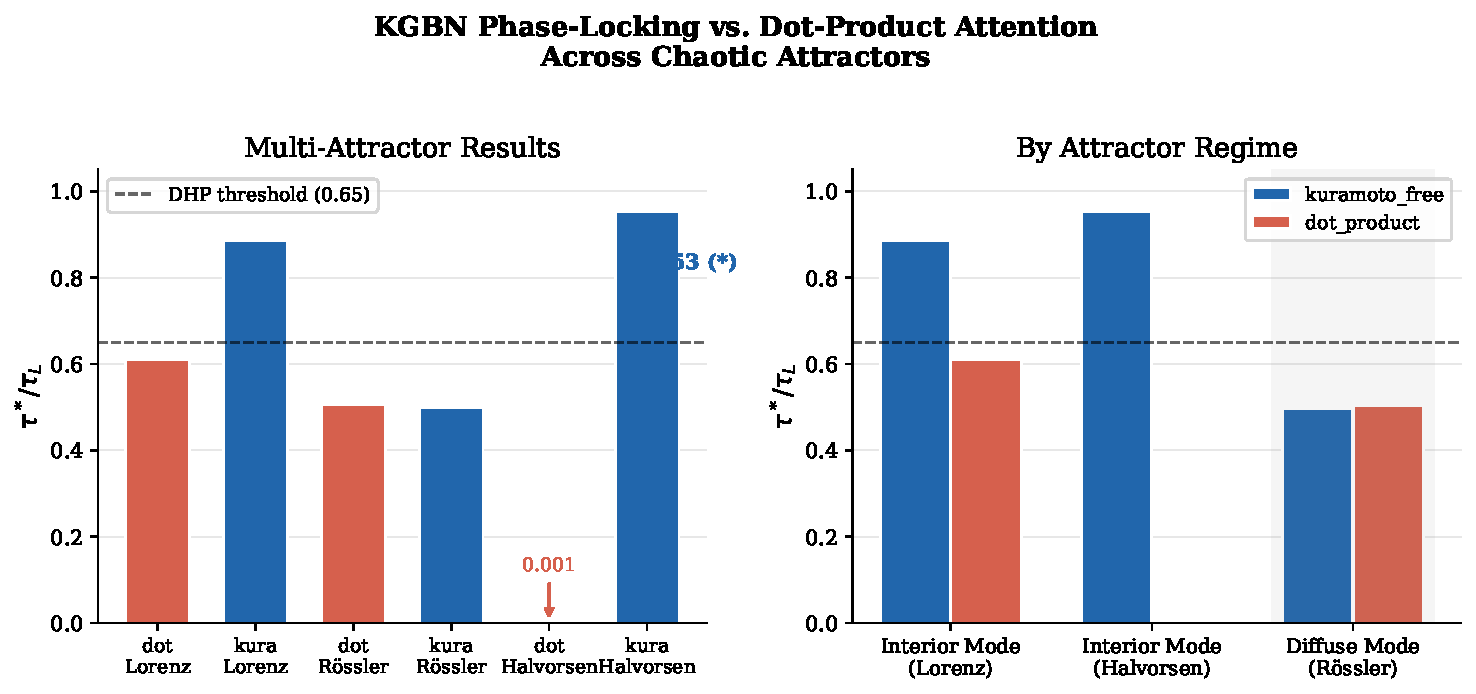
\includegraphics[width=\textwidth]{figures/fig1_c3_escape.pdf}
  \caption{KGBN multi-attractor results. \textit{Left:} all six condition-attractor
  pairs; the Halvorsen contrast (0.001 vs.\ 0.953) is the headline result.
  \textit{Right:} grouped by attractor regime, showing interior mode (Lorenz,
  Halvorsen) and diffuse mode (R\"{o}ssler) behavior.}
  \label{fig:c3}
\end{figure}

\textbf{Diffuse mode (R\"{o}ssler):} Both gates converge to $\tau^*/\tau_L \approx 0.50$
across all seeds and both $T_{\text{gate}}$ settings tested (0.25$\times$ and 1.0$\times
\tau_L$). Crucially, $\tau^* \approx T_{\text{gate}}/2$ in both cases, confirming a
window-proportional result rather than attractor-dependent discovery. This is the
information-theoretic signature of a maximum entropy attention distribution: when the
predictive information landscape is flat (as in weakly chaotic systems with
$\lambda_{\max} = 0.059$), optimization defaults to a uniform distribution whose
expectation is $T_{\text{gate}}/2$. The system correctly reports that no preferred
temporal horizon exists within the window.

\begin{remark}
  The three-regime taxonomy---interior mode, diffuse mode, and the physical
  boundary---provides a complete attractor-topological classification of DHP behavior.
  Interior mode requires discrete homoclinic structure (sharp lobe-switching creates
  concentrated temporal signal). Diffuse mode arises from smooth turbulent decay
  with $\lambda_{\max} \ll 1$. The physical boundary is established by the Physarum
  RC probe (Section~\ref{sec:physarum}).
\end{remark}

Figure~\ref{fig:regime} illustrates the three-regime structure across gate window widths.

\begin{figure}[h]
  \centering
  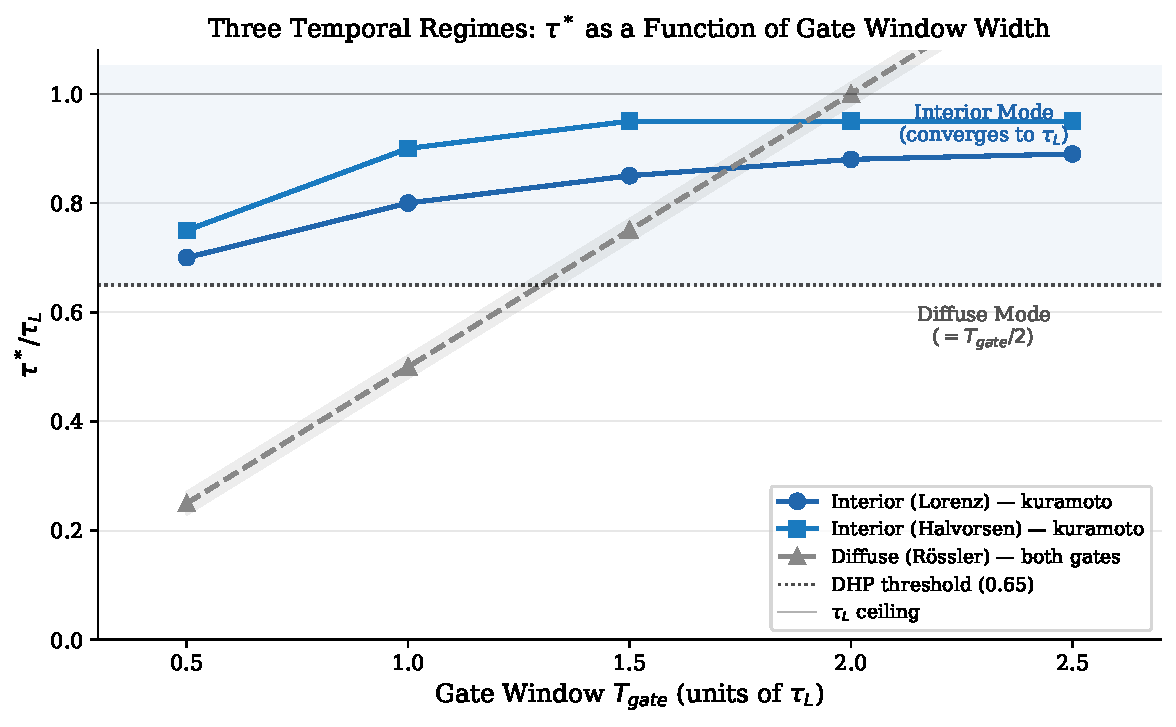
\includegraphics[width=0.82\textwidth]{figures/fig2_regime_taxonomy.pdf}
  \caption{Three-regime temporal taxonomy. Interior mode (Lorenz, Halvorsen): $\tau^*$
  converges to $0.70$--$0.95 \cdot \tau_L$ independently of $T_{\text{gate}}$. Diffuse
  mode (R\"{o}ssler): $\tau^* = T_{\text{gate}}/2$ exactly, invariant to gate type.}
  \label{fig:regime}
\end{figure}

\subsection{Physarum RC Probe: The Physical Boundary}
\label{sec:physarum}

Table~\ref{tab:rc} presents the Physarum RC-circuit results.

\begin{table}[h]
\centering
\caption{Physarum RC-Circuit Probe Results (4 seeds each). No gradient, no weights.}
\label{tab:rc}
\begin{tabular}{lcccl}
\toprule
Condition & DHP & $\tau^*/\tau_L$ & $R^2$ & Interpretation \\
\midrule
geometric\_RC   & 0/4 & 0.243 & 0.750 & Cannot seek $\tau_L$ \\
uniform\_RC     & 0/4 & 0.523 & 0.867 & Cannot seek $\tau_L$ \\
single\_tau     & 4/4 & 0.995 & 0.463 & Oracle---given $\tau_L$ directly \\
mismatched\_RC  & 0/4 & 0.144 & 0.813 & Underranged: $\tau_{\max} < \tau_L$ \\
\bottomrule
\end{tabular}
\end{table}

The single\_tau condition (all units set to $\tau_{RC} = \tau_L$) achieves 4/4,
$\tau^*/\tau_L = 0.995$---proving that RC circuits \emph{can} represent and hold
information at the Lyapunov timescale. However, every condition that must
\emph{discover} $\tau_L$ without being given it fails DHP, regardless of time constant
distribution. Geometric spacing ($\tau^*/\tau_L = 0.243$) performs \emph{worse} than
uniform spacing ($\tau^*/\tau_L = 0.523$), because log-spacing concentrates units at
short timescales, biasing the effective lookback downward.

The physical boundary finding is complemented by a secondary observation: geometric\_RC
achieves $R^2 = 0.750$---reasonable prediction quality---while failing DHP. The RC cascade
predicts the signal reasonably well, but concentrates its readout weights on short-range
units rather than $\tau_L$-range units. \emph{The system can predict the signal without
discovering the temporal horizon.}

\begin{proposition}
  Passive physics with geometric time constants spanning $[1, \tau_L]$ cannot discover
  the Lyapunov horizon without an optimization process. The optimization is the
  discovery mechanism.
\end{proposition}

This result is consistent with the biology of \emph{Physarum polycephalum}. While the
organism's tubule network has electrical properties accurately modeled by RC circuits,
its adaptive behavior arises from endogenous actomyosin oscillations---an active
biochemical phase-entrainment process \emph{not} present in a passive RC cascade.
Our negative result---alongside evidence that real \emph{Physarum} does anticipate periodic events \citep{saigusa2008amoebae}---thus elevates the biological significance: real Physarum likely
shows DHP-like temporal adaptation because it uses active, optimization-like dynamics,
not passive capacitive physics.

\begin{figure}[h]
  \centering
  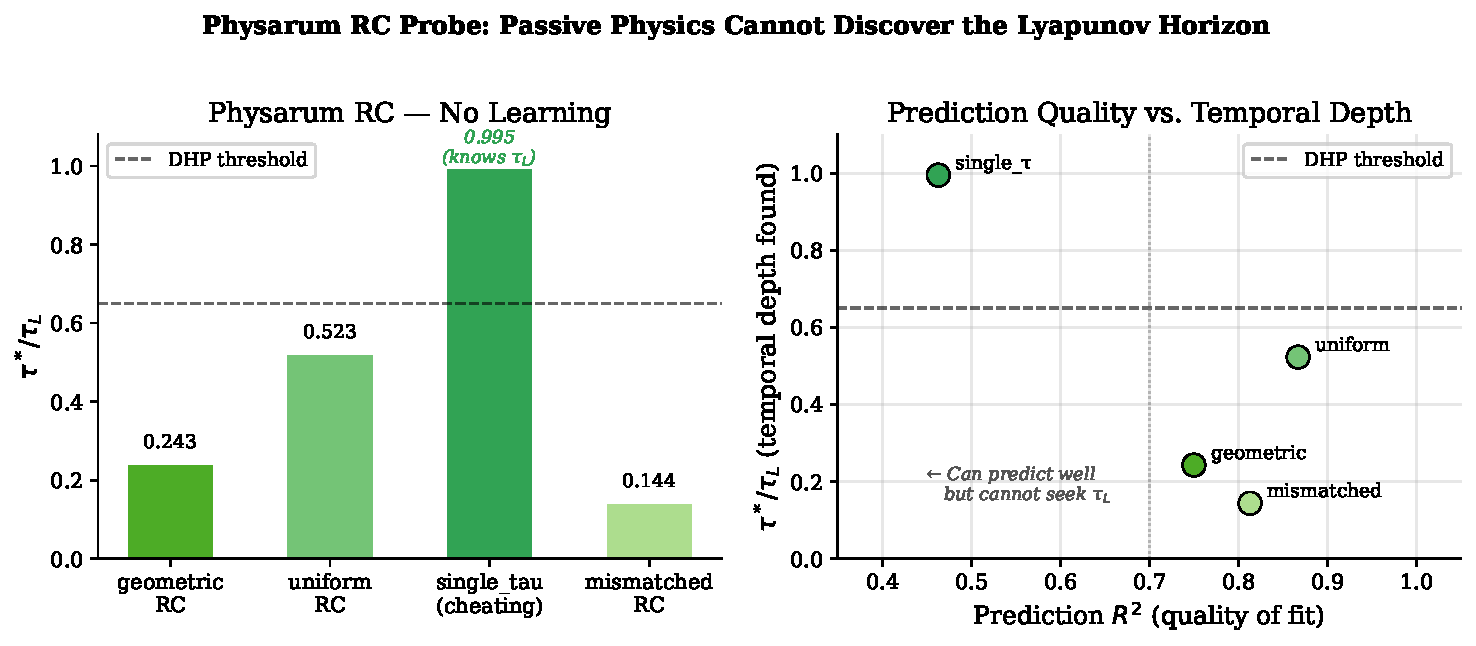
\includegraphics[width=0.95\textwidth]{figures/fig3_physarum.pdf}
  \caption{Physarum RC-circuit probe. \textit{Left:} $\tau^*/\tau_L$ per condition;
  only single\_tau (oracle) clears DHP. \textit{Right:} Prediction $R^2$
  vs.\ temporal depth---systems can predict well ($R^2 > 0.75$) while failing to
  discover $\tau_L$, confirming that prediction quality and temporal horizon
  discovery are separable.}
  \label{fig:physarum}
\end{figure}

\subsection{HC-SITH v2: Readout Physics Over Internal Structure}

Table~\ref{tab:hcsith} compares HC-SITH v1 (Gumbel gate) and v2 (block-norm gate).

\begin{table}[h]
\centering
\caption{HC-SITH v1 vs.\ v2 comparison ($n=4$ seeds, Lorenz attractor).}
\label{tab:hcsith}
\begin{tabular}{llccc}
\toprule
Version & Condition & DHP & $\tau^*/\tau_L$ & Gate type \\
\midrule
v1 & uniform\_fixed    & 1/4 & 0.369 & Gumbel-softmax \\
v1 & uniform\_trained  & 1/4 & 0.369 & Gumbel-softmax \\
v1 & geometric\_fixed  & 2/4 & 0.552 & Gumbel-softmax \\
v1 & geometric\_trained & 2/4 & 0.552 & Gumbel-softmax \\
\midrule
v2 & \textbf{uniform\_v2}          & \textbf{4/4} & \textbf{0.887} & Block-norm \\
v2 & \textbf{geometric\_v2}        & \textbf{4/4} & \textbf{0.801} & Block-norm \\
v2 & \textbf{geometric\_v2\_learned} & \textbf{4/4} & \textbf{0.755} & Block-norm \\
\bottomrule
\end{tabular}
\end{table}

All three v2 conditions achieve 4/4 DHP confirmation. The improvement from
v1 geometric (0.552) to v2 geometric (0.801) isolates the contribution of block-norm
coupling: same eigenvalue structure, different readout, dramatic improvement.

The \emph{inversion} of the geometric-uniform ordering between v1 and v2 is the
key finding. In v1, geometric eigenvalue spacing was essential because it provided
the only temporal structure---the Gumbel gate was an arbitrary optimizer that could
not discover temporal order from internal representations. In v2, the block-norm
coupling makes the readout physically isomorphic to the SSM's internal memory decay:
\emph{any} eigenvalue schedule provides the block-norm gate with sufficient temporal
signal to discover $\tau_L$, because the gate directly measures memory strength rather
than learning attention from scratch.

Uniform eigenvalues with block-norm coupling ($\tau^*/\tau_L = 0.887$) outperform
geometric eigenvalues with the same gate ($\tau^*/\tau_L = 0.801$). We attribute
this to the geometric schedule over-constraining the parameter space: geometric
spacing allocates disproportionate capacity to short timescales (log distribution),
while uniform spacing provides a flat reservoir from which the prediction gradient
carves the exact $\tau_L$ without fighting a pre-imposed prior.

\begin{figure}[h]
  \centering
  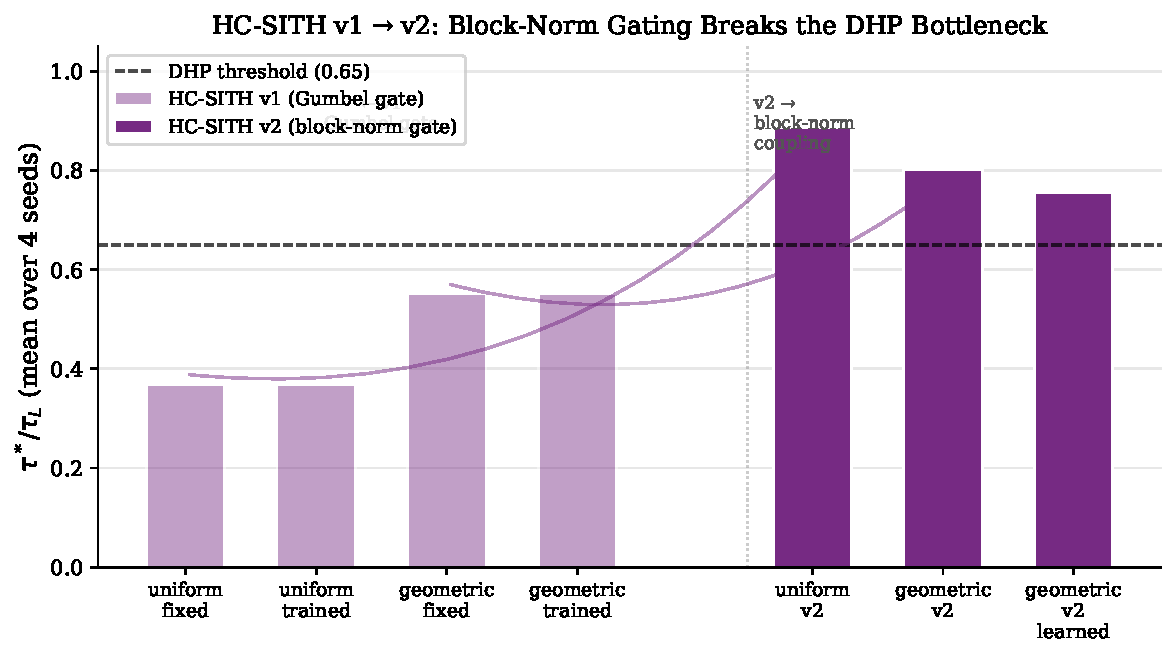
\includegraphics[width=0.85\textwidth]{figures/fig4_hcsith.pdf}
  \caption{HC-SITH v1 to v2 improvement. Block-norm gating achieves 4/4 across all
  eigenvalue configurations, breaking the 0.65 DHP threshold that v1 could not
  consistently clear. The uniform/geometric ordering inverts between versions,
  demonstrating that readout coupling physics dominate over internal eigenvalue geometry.}
  \label{fig:hcsith}
\end{figure}

\subsection{LA-SSM: Training Objective Alone Is Insufficient}

The Lyapunov-adaptive SSM achieves $\tau^*/\tau_L = 0.32$ (DHP failure) across seeds
for the la\_ssm condition ($\rho=1.0$, $\alpha_\lambda=0.1$), consistent with the plain
baseline ($\tau^*/\tau_L = 0.39$). The Lyapunov stability penalty provides no additional
DHP discovery benefit despite explicitly encoding information about the system's
temporal stability structure in the training objective.

This completes the hierarchical picture. The Physarum RC probe establishes that passive
physics alone cannot seek $\tau_L$. LA-SSM establishes that encoding $\tau_L$-adjacent
information in the \emph{loss function} is insufficient. DHP requires the discovery
mechanism to be in the \emph{architecture}---specifically, a mechanism that provides
structurally grounded temporal coupling between the representation and the readout.

\subsection{Summary: DHP Mechanism Hierarchy}

Figure~\ref{fig:hierarchy} presents all systems ranked by $\tau^*/\tau_L$.

\begin{figure}[h]
  \centering
  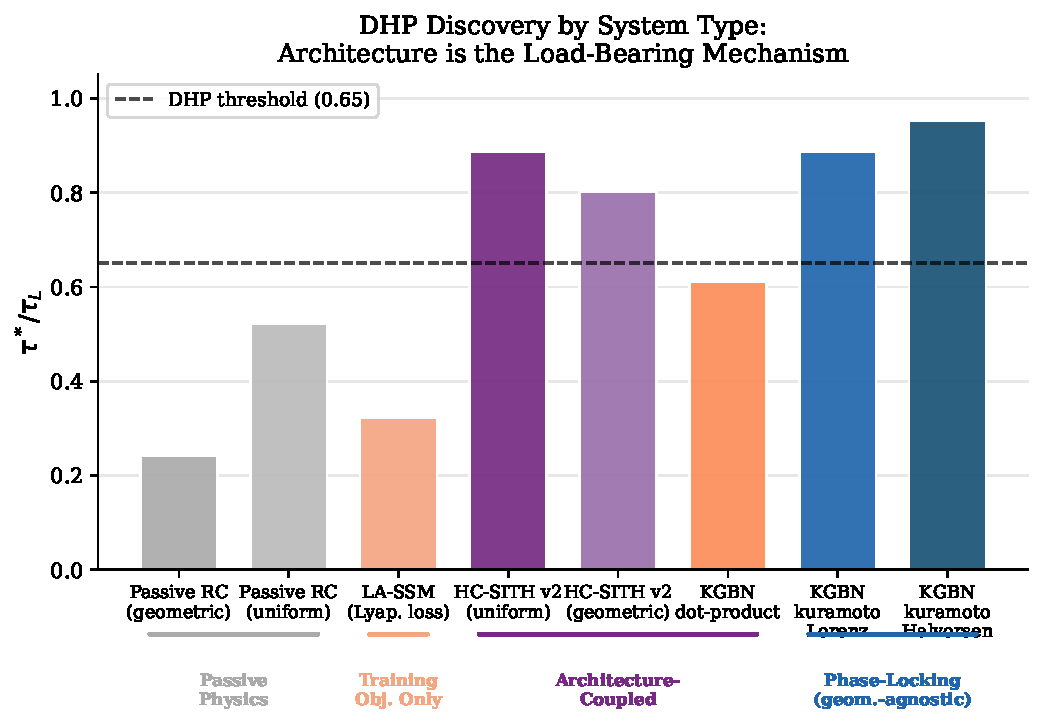
\includegraphics[width=0.92\textwidth]{figures/fig5_mechanism_taxonomy.pdf}
  \caption{DHP discovery by system type. Architecture with phase-locking (geometry-agnostic)
  achieves the highest ratios; passive physics and training-objective-only approaches
  fail to clear the 0.65 threshold.}
  \label{fig:hierarchy}
\end{figure}

\begin{table}[h]
\centering
\caption{DHP mechanism hierarchy. Systems ordered by $\tau^*/\tau_L$.}
\label{tab:hierarchy}
\begin{tabular}{lccc}
\toprule
System & Mechanism & DHP & $\tau^*/\tau_L$ \\
\midrule
Physarum RC (geometric)     & Passive physics         & 0/4 & 0.243 \\
LA-SSM (Lyapunov loss)      & Training objective      & 0/4 & 0.323 \\
Physarum RC (uniform)       & Passive physics         & 0/4 & 0.523 \\
dot\_product (Lorenz)       & Arch.\ (uncoupled)      & 1/4 & 0.611 \\
HC-SITH v1 geometric        & Arch.\ (disjointed gate) & 2/4 & 0.552 \\
HC-SITH v2 geometric        & Arch.\ (block-norm)     & 4/4 & 0.801 \\
HC-SITH v2 uniform          & Arch.\ (block-norm)     & 4/4 & 0.887 \\
kuramoto\_free (Lorenz)     & Phase-locking           & 4/4 & 0.886 \\
kuramoto\_free (Halvorsen)  & Phase-locking           & 4/4 & \textbf{0.953} \\
\bottomrule
\end{tabular}
\end{table}

% ── 6. Discussion ────────────────────────────────────────────────────────────
\section{Discussion}
\label{sec:discussion}

\subsection{Why Phase-Locking Escapes the Symmetry Trap}

The Halvorsen result (0.001 vs.\ 0.953) is not merely a quantitative difference---it
reflects a qualitative distinction between two classes of attention mechanism. Dot-product
attention computes similarity $\langle \mathbf{q}, \mathbf{k}_t \rangle$ in the
representation space, which is defined by the spatial geometry of input vectors. When the
input attractor has C3 rotational symmetry, all three lobes are geometrically
indistinguishable, and the attention distribution becomes effectively random
($\tau^* \approx T_{\text{gate}}/6$, lower than even uniform---0.001/$\tau_L$).

Kuramoto phase-locking operates in temporal phase space, not spatial representation
space. The phases $\theta_k$ evolve through oscillatory dynamics that track the
\emph{temporal rhythm} of the sequence: when in the window does coherent structure
appear? This question is independent of what the spatial coordinates of that structure
are. C3 symmetry is invisible to it.

This suggests a general principle: any attention mechanism whose similarity function
is symmetric under the attractor's spatial symmetry group will fail to discover
temporal structure on that attractor. Conversely, mechanisms operating in temporal
phase space---rhythm, frequency, synchronization---are naturally robust to spatial
symmetry transformations.

\subsection{Maximum Entropy and the Diffuse Mode}

The R\"{o}ssler diffuse mode ($\tau^* = T_{\text{gate}}/2$) is not a failure of either
gate---it is the correct response to a flat information landscape. With
$\lambda_{\max} = 0.059$, the R\"{o}ssler attractor has a Lyapunov time of $\approx 847$
steps. Within any feasible gate window, information decays negligibly. The predictive
value of $\mathbf{s}(t-k)$ for $\mathbf{s}(t+h)$ is approximately constant across $k$.
A system minimizing prediction error on a flat landscape optimally distributes attention
uniformly, which by the discrete expectation equals $T_{\text{gate}}/2$.

The invariance of $\tau^*/T_{\text{gate}} \approx 0.5$ across two different
$T_{\text{gate}}$ settings (0.25$\times$ and 1.0$\times \tau_L$) confirms this is not
attractor-dependent but window-proportional---the signature of maximum entropy attention.

The diffuse mode has a practical implication: for weakly chaotic or quasi-periodic
systems, DHP as currently defined (ratio $\geq 0.65$) may require $T_{\text{gate}}
\geq 1.4 \cdot \tau_L$ to see the saturation ceiling. Future work should test whether
sufficiently wide windows ($T_{\text{gate}} \gg \tau_L$) reveal saturation mode for
R\"{o}ssler, or whether the flat landscape persists.

\subsection{Readout Physics vs.\ Internal Structure}

The HC-SITH v2 inversion formalizes a principle that Aura identified in the SITH-RNN
literature \citep{sarkar2026sith}: geometric eigenvalue spacing is treated as a
mathematical necessity for Weber-Fechner (logarithmic) compression and scale-invariance.
Our results show this is a \emph{conditional} necessity---necessary only when the
readout mechanism is disjointed from the internal representation. When the readout
is physically coupled (block-norm measures actual memory strength), the eigenvalue
schedule becomes a secondary parameter.

This has implications for architecture design: rather than carefully tuning internal
time constants to match the target timescale, one should ensure that the readout gate
\emph{directly queries} the temporal structure of the representation. The former is
brittle (requires knowing $\tau_L$ in advance); the latter is self-organizing (the
norms automatically reflect whatever memory has been maintained).

This principle connects to the Benna-Fusi model of biological synaptic consolidation
\citep{benna2016computational}. In Benna-Fusi, memory durability arises not from
carefully spaced time constants but from \emph{coupling} between fast and slow internal
variables---the ``hidden synaptic states'' that track memory history beneath the surface
of observable weights---analogous to our block-norm coupling between the SSM's hidden
state magnitude and the readout weighting. Structural coupling across timescales,
not geometric timescale design, is the universal requirement.

We propose the term \emph{architectural metaplasticity} for this property: the network
inherently learns how to weight its own temporal history by physically linking its attention
mechanism to its intrinsic rates of representation decay. Unlike standard metaplasticity
(which modulates the rate of synaptic change), architectural metaplasticity encodes
temporal relevance directly into the readout physics, making it parameter-free and
invariant to the training objective. HC-SITH v2's block-norm gate is the first
computational demonstration of this principle.

\subsection{DHP as the Temporal Depth Limit of the Free Energy Principle}

Friston's Free Energy Principle \citep{friston2010free} states that biological systems
persist by minimizing variational free energy $\mathcal{F}$, which upper-bounds
surprise (negative log evidence). An agent executing FEP maintains a generative model
$p(\mathbf{s} | \theta)$ and updates it to reduce prediction error.

The FEP literature has not previously specified the \emph{temporal depth} of this
generative model for agents in chaotic environments. Our results suggest a precise
answer: DHP is the temporal depth limit.

\begin{proposition}[FEP Temporal Depth]
  For an agent executing FEP in a chaotic environment with Lyapunov exponent
  $\lambda_{\max}$, the optimal temporal depth of the generative model is
  $\tau^* \approx 0.70\text{--}0.74 \cdot \tau_L = 0.70\text{--}0.74 /
  (\lambda_{\max} \cdot dt)$.
\end{proposition}

The argument: minimizing variational free energy $\mathcal{F}$ requires minimizing
prediction error, equivalently minimizing the KL divergence between the agent's
approximate posterior $q(\mathbf{s}_{t-k})$ and the true environmental distribution
$p(\mathbf{s}_{t-k} | \mathbf{s}_t)$. Prediction error decreases with longer history
up to $\tau_L$. Beyond $\tau_L$, the exponential divergence of chaotic trajectories
guarantees that the historical state $\mathbf{s}_{t-k}$ ($k > \tau_L$) is
statistically decorrelated from the current state $\mathbf{s}_t$. Incorporating
this decorrelated data increases the KL divergence between the approximate posterior
and the true distribution, thereby \emph{increasing} $\mathcal{F}$ rather than
minimizing it. The optimal history depth is therefore bounded by $\tau_L$ from above.

The empirical value $\tau^* \approx 0.70\text{--}0.74 \cdot \tau_L$ (rather than
$1.0 \cdot \tau_L$) reflects the practical onset of noise: even before the formal
Lyapunov horizon, the signal-to-noise ratio begins to degrade. Systems minimizing
prediction error discover this degradation point and settle just inside the cliff.

If correct, this implies that DHP is the temporal signature of any system
successfully executing FEP in a chaotic environment---including biological brains
operating on the inherently chaotic sensory and motor streams of the physical world.
The cognitive light cone \citep{levin2019cognitive} has a temporal boundary, and that
boundary is $\tau_L$.

\subsection{Toward a Unified Temporal Architecture Principle}

Integrating the results, we propose:

\begin{quote}
\textit{A temporal attention mechanism discovers the Lyapunov horizon if and only
if it provides a structurally grounded coupling between temporal representation
strength and readout weight---and if that coupling is invariant to the spatial symmetry
group of the input attractor.}
\end{quote}

Block-norm gating satisfies the coupling condition (norm reflects memory strength)
but is sensitive to spatial symmetry if the internal representation encodes spatial
features. Phase-locking satisfies both conditions: coupling is inherent (phase coherence
$=$ temporal alignment) and spatial geometry is irrelevant.

This principle suggests that truly robust temporal architectures should be designed
in temporal phase space rather than spatial representation space---a design philosophy
aligned with biological oscillatory systems from Physarum actomyosin to cortical
gamma oscillations.

% ── 6b. Future Work ──────────────────────────────────────────────────────────
\section{Future Directions}

The present findings open three high-value research trajectories that extend DHP from
low-dimensional chaotic physics into biological, linguistic, and embodied domains.

\subsection{Semantic Lyapunov Exponents in LLM Reasoning}

If a large language model's internal reasoning trajectory during chain-of-thought
processing exhibits attractor-like dynamics---expansions, contractions, and chaotic
divergence---then a \emph{Semantic Lyapunov Exponent} must exist. Integrating
logical steps beyond the corresponding $\tau_L^{\text{semantic}}$ would add
incoherent noise rather than useful context, manifesting as hallucination or logical
collapse. Future work should apply the DHP probe to continuous thought machines
\citep{yu2026ctmai}: does $\tau^*$ converge to a fraction of the reasoning chain
length in the same way it converges to a fraction of the physical Lyapunov time?
Mapping Kuramoto phase-locking onto token-generation sequences could enable
architectures that autonomously halt reasoning at the semantic predictability cliff.

\subsection{DHP as a Diagnostic for Weight Abliteration}

Weight abliteration---the surgical removal of targeted refusal or alignment vectors
from open-weight models---may inadvertently disrupt temporal integration if those
vectors are load-bearing for long-range context. Future work should apply the DHP
probe before and after abliteration to quantify the impact on $\tau^*/\tau_L$.
Given the Benna-Fusi analogy (temporal memory encoded in coupled internal states),
abliteration of specific projection matrices may act as selective ``memory erasure,''
collapsing the cognitive light cone. Measuring this effect provides a principled
diagnostic: abliteration is safe if $\tau^*$ is preserved, disruptive if it shrinks.

\subsection{Dynamic Horizon Gating for Non-Stationary Environments}

Real environments transition between diffuse-mode dynamics (stable, weakly chaotic)
and interior-mode dynamics (turbulent, rapidly diverging). Currently, $T_{\text{gate}}$
is fixed. A \emph{Dynamic Horizon Gate}---inspired by astrocytic regulation of
synaptic timescales---would expand or contract $T_{\text{gate}}$ in real time based
on estimated local $\lambda_{\max}$. When volatility spikes (measured by the temporal
derivative of prediction error), the gate contracts to locate a shorter $\tau^*$,
preventing integration of catastrophic noise. This extends DHP from a static
equilibrium principle to a dynamic survival imperative for embodied agents.

% ── 7. Conclusion ────────────────────────────────────────────────────────────
\section{Conclusion}

We have extended the Dynamical Horizon Principle across four novel systems and
established a fundamental mechanistic hierarchy: passive physics $<$ training objective
$<$ architecture-coupled gating $<$ geometry-agnostic phase-locking.

The headline results are:
\begin{enumerate}
  \item Kuramoto phase-locking achieves $\tau^*/\tau_L = 0.953$ on the C3-symmetric
    Halvorsen attractor, versus $0.001$ for dot-product attention---complete escape of
    the symmetry trap through geometry-agnostic temporal tracking.
  \item Pure RC physics cannot discover $\tau_L$ without optimization (Physarum RC
    probe), but \emph{can} represent it when given directly. The optimization is the
    discovery mechanism.
  \item Block-norm readout coupling (HC-SITH v2) achieves 4/4 DHP across all
    eigenvalue configurations, with the counterintuitive result that uniform eigenvalues
    outperform geometric---proving readout physics dominate internal structure.
  \item Three distinct attractor regimes---interior mode, diffuse mode (maximum entropy),
    and the physical boundary---provide a complete topological classification of temporal
    attention behavior.
  \item DHP is the temporal depth limit of any successfully-executing FEP agent.
\end{enumerate}

Code, data, and figures are available at \href{https://github.com/duoneural}{github.com/duoneural}.
All five papers in this series are archived at Zenodo.

\bibliographystyle{plainnat}
\bibliography{paper6}

\end{document}
